\documentclass[12pt]{beamer}
\usepackage[utf8]{inputenc}
\usepackage[T1]{fontenc}
\usepackage{lmodern}
%\usetheme{Malmoe}
\usetheme{Ilmenau}
\usecolortheme{orchid}
\usepackage{graphicx}
\usepackage{newverbs}

\newverbcommand{\tc}{\color{blue}}{}

%\usebackgroundtemplate{\includegraphics[width=\paperwidth,height=\paperheight]{./images/background.jpg}}

\begin{document}
	\author{Lukáš Růžička (lruzicka@redhat.com)}
	\title{Bugzilla Kills Godzilla}
	\subtitle{or How to report bugs the useful way}
	\titlegraphic{
\includegraphics[height=2cm]{buggie.png}}
	\institute{Fedora QE}
	\date{}
%	\subject{Fedora 29}
	%\setbeamercovered{transparent}
	%\setbeamertemplate{navigation symbols}{}

\begin{frame}[plain]
	\maketitle 
\end{frame}

\section{Introduction}

\begin{frame}{What is Bugzilla?}
Bugzilla is a bug-tracking (issue-tracking) system. Among the most important features are:

\begin{itemize}
\item open source
\item powerful bug tracking
\item highly configurable
\item history aware
\item robust and stable
\item secure
\item various interfaces (configurable and localisable)
\end{itemize}

More at {\color{blue}\url{www.bugzilla.org}}.
\end{frame}

\begin{frame}{Red Hat Bugzilla}
Bugzilla is the bug-tracking system used at Red Hat. It is available to everyone (customers, collaborators, developers, QAs and more) interested in:

\begin{itemize}
	\item Red Hat products
	\item JBoss products
	\item Fedora products
	\item Community projects
	\item Internal products
\end{itemize}

Red Hat Bugzilla lives at {\color{red}\url{bugzilla.redhat.com}}.
\end{frame}

\begin{frame}{Why bug tracking?}

By tracking you bugs, you can

\begin{itemize}
	\item receive information about a problem
	\item organize your time, plan, and estimate
	\item cooperate with others
	\item share knowledge and ideas
	\item see the progress
	\item find a solution.
\end{itemize}
\end{frame}

\begin{frame}{Why you should think about reporting bugs?}
Reporting bugs is an important activity because you
\begin{itemize}
	\item want a problem fixed
	\item have a unique hardware and setting
	\item have a new idea
	\item have different needs and expectations
	\item want to keep people informed
\end{itemize}
If you report bugs, your will contribute a lot with just a little cost.
\end{frame}

\section{Reporting bugs}

\begin{frame}{What could be a bug?}
You would like to report a bug anytime you find out that something is not right. For example, when the program:
\begin{itemize}
	\item does not start
	\item keeps crashing
	\item behaves incorrectly
	\item reports errors
	\item has problems with user interface
	\item lacks some features
	\item and more
\end{itemize}
\end{frame}

\begin{frame}{Before you report}
It is good to report bugs when you have some information about them. You should be able to describe

\begin{itemize}
	\item what happened
	\item when 
	\item how 
	\item how often
	\item why (if possible)
	\item why it should not have happened
\end{itemize}	
\end{frame}

\begin{frame}{How to reproduce a bug?}
	Reproducing the bug is a very important thing. If you cannot reproduce it, tracking it down can be impossible.
	\begin{itemize}
		\item Try to make the bug happen again.
		\item Learn the steps that lead to the bug.
		\item Try changing some of the steps and see if it changes things.
	\end{itemize}
\end{frame}

\begin{frame}{Getting and providing info}
If your bug report should be good, you have to collect some info to provide, for example:
\begin{itemize}
	\item system logs
	\item system info
	\item how to reproduce the bug
	\item screenshots
	\item videos
\end{itemize}
\end{frame}

\begin{frame}{ABRT}
The \textbf{Automatic Bugzilla Reporting Tool} is a service that monitors your computer and analyzes problems.
\begin{itemize}
	\item installed by default
	\item runs as a service
	\item collects data
	\item makes reporting easier
	\item sometimes useless
\end{itemize}
\end{frame}

\begin{frame}{journalctl}
\textbf{journalctl} is a front-end to a service that collects the majority of logs of the system. You can filter the logs using various options.
\begin{description}
	\item[journalctl -b] shows logs from the latest boot
	\item[journalctl -u] shows logs from a certain system unit
	\item[journalctl -f] shows latest logs and continuously shows new records
	\item[journalctl -S -U] shows logs between certain time
\end{description}
See \texttt{man journalctl} for more info.
\end{frame}

\begin{frame}{Collecting logs}
Applications and services use logging to text files to keep track of all their activities. These logs can be examined, to see what went wrong. Logs can be located:
\begin{itemize}
	\item journalctl
	\item \texttt{/var/log/*}
	\item other locations (check settings)
\end{itemize}	
\end{frame}

\section{Using Bugzilla}
\begin{frame}{New at Bugzilla}
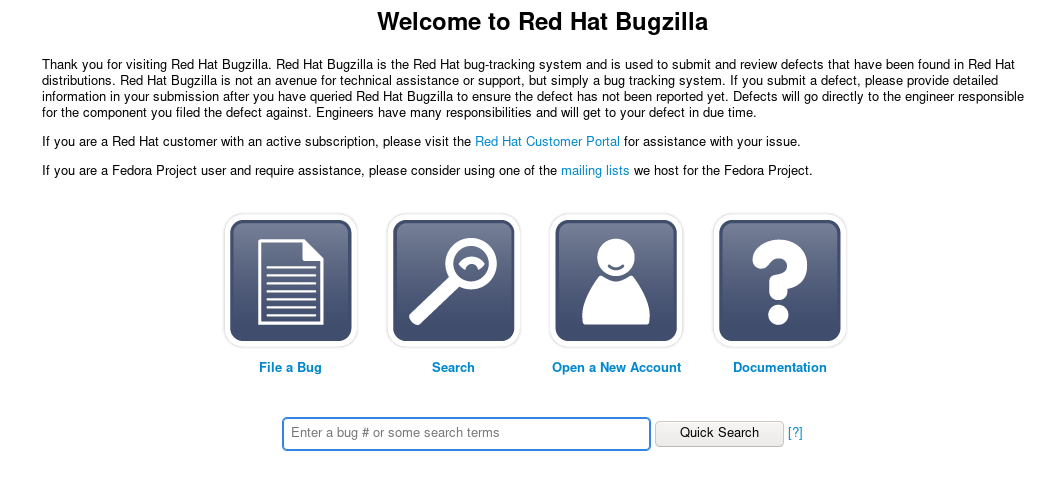
\includegraphics[width=10cm]{images/bz_new.png}
\end{frame}

\begin{frame}{Logged into Bugzilla}
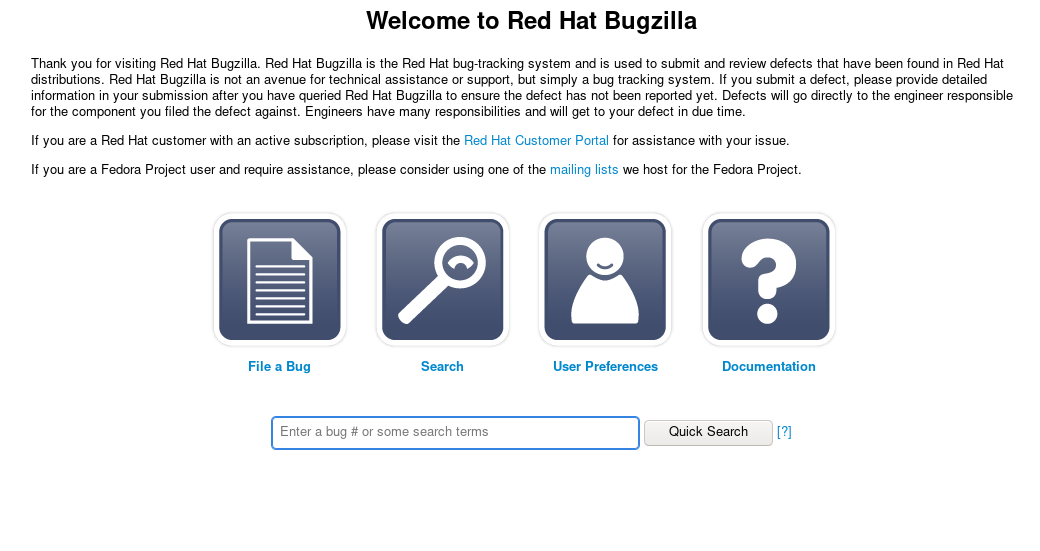
\includegraphics[width=10cm]{images/bz_logged.png}
\end{frame}

\begin{frame}{Classify the bug}
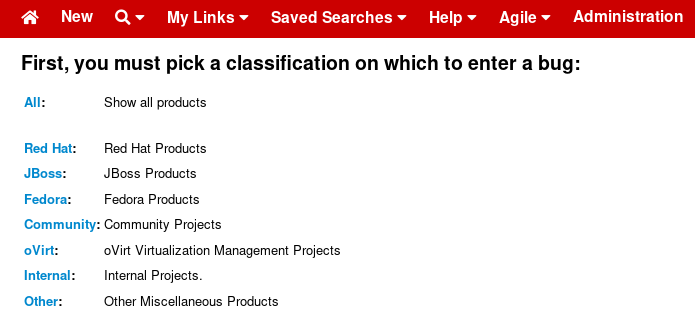
\includegraphics[width=10cm]{images/bz_classification.png}
\end{frame}

\begin{frame}{Choose the correct product}
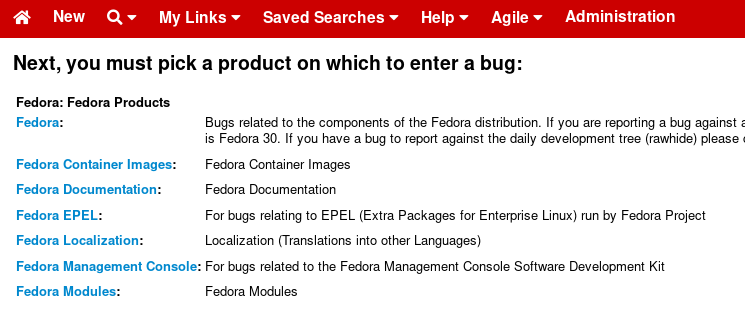
\includegraphics[width=10cm]{images/bz_product.png}
\end{frame}

\begin{frame}{File the bug (part 1)}
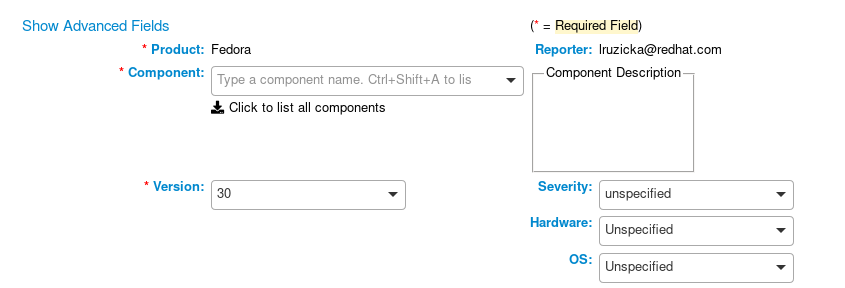
\includegraphics[width=10cm]{images/bz_header.png}
\end{frame}

\begin{frame}{File the bug (part 2)}
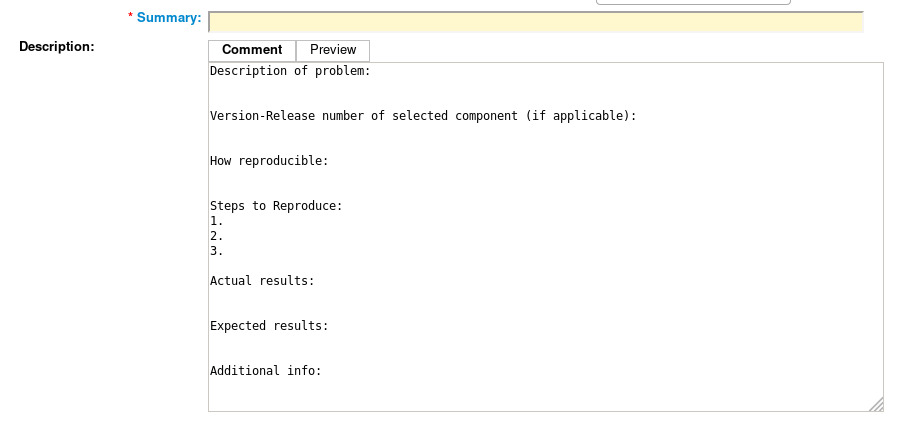
\includegraphics[width=10cm]{images/bz_description.png}
\end{frame}

\begin{frame}{Description of problem}
\begin{itemize}
	\item What is the problem?
	\item When does it appear?
	\item How much does it affect work?
	\item Why is it a problem?
	\item others
\end{itemize}
\end{frame}

\begin{frame}{Version of selected component}
Provide the version number of the problematic components and also of the affected components.
\begin{itemize}
	\item \textbf{About} menu in GUI
	\item \texttt{-v} or \texttt{--version} option on CLI (or \texttt{man})
	\item \texttt{rpm -q} for installed packages
	\item \texttt{dnf info} for installed and available packages
\end{itemize}
\end{frame}

\begin{frame}{How reproducible}
\begin{itemize}
	\item Always
	\item Sometimes
	\item Under certain conditions -- describe them
	\item Heisenbug 
\end{itemize}
\end{frame}

\begin{frame}{Steps to reproduce}
Procedure that leads to reproducing the bug.
\begin{itemize}
	\item One activity in one step.
	\item Do not skip steps, even if you think the step is obvious.
	\item Be exact and detailed.
\end{itemize}
Others want to see that bug, too. 
\end{frame}

\begin{frame}{Results}
\begin{description}
	\item[Actual] -- what is the result of the current behaviour
	\item[Expected] -- how you think the system should behave
\end{description}
\end{frame}

\begin{frame}{File the bug (part 3)}
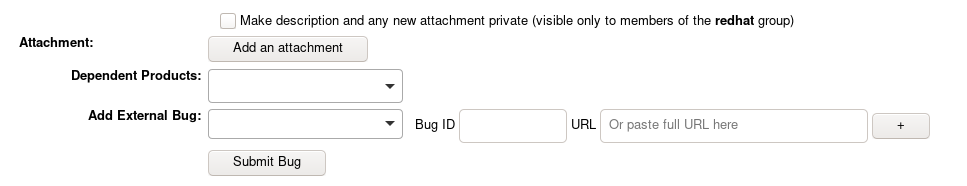
\includegraphics[width=10cm]{images/bz_footer.png}
\end{frame}

\begin{frame}{No clue about anything?}

{\Large File the bug anyway!}
\end{frame}


\end{document}